\documentclass{beamer}
\usepackage{graphicx}
\usepackage{xcolor}
\usepackage{tikz}
\usepackage{amsmath}
\DeclareGraphicsExtensions{.png,.pdf,.jpg,.jpeg}

\definecolor{purpleblue}{RGB}{80, 80, 180}
\definecolor{lightgray}{RGB}{230, 230, 230}
\definecolor{novelPurple}{RGB}{98, 54, 255}
\definecolor{darkgray}{RGB}{50, 50, 50}
\definecolor{softPurple}{RGB}{180, 170, 255}
\definecolor{softGray}{RGB}{235, 235, 245}
\definecolor{lightText}{RGB}{90, 90, 110}
\graphicspath{{static/unit4/}{./}}

\usetheme{Madrid}
\usecolortheme{dolphin}

\setbeamerfont{title}{size=\Large,series=\bfseries}
\setbeamerfont{frametitle}{size=\LARGE,series=\bfseries}
\setbeamercolor{frametitle}{fg=white, bg=novelPurple}
\setbeamercolor{title}{fg=white, bg=purpleblue}

\title[SAT Unit 4.1]{\textbf{SAT Unit 4.1 \\Volume and Area}}
\author{\textbf{Jack Zeng}}
\institute{\textcolor{white}{\textbf{Novel Prep}}}
\date{\today}

\begin{document}

\begin{frame}
    \titlepage
    \vfill
    \begin{flushright}
        \textcolor{purpleblue}{\Huge \textbf{Novel Prep}}
    \end{flushright}
\end{frame}

\begin{frame}
    \begin{tikzpicture}[remember picture, overlay]
        \shade[top color=softPurple, bottom color=softGray]
            (current page.north west) rectangle (current page.south east);
        \fill[white, opacity=0.3] (current page.center) circle (4cm);
        \node[align=center] at (current page.center) {
            {\Huge\bfseries\textcolor{purpleblue}{Novel Prep}} \\[0.5cm]
            {\Large\itshape\textcolor{lightText}{Excellence in SAT Prep}}
        };
        \foreach \x in {1,2,3,4,5} {
            \fill[purpleblue, opacity=0.2] (rand*10-5, rand*7-3.5) circle (0.1+\x*0.05);
        }
    \end{tikzpicture}
\end{frame}

\begin{frame}{Overview}
    \tableofcontents
\end{frame}


\begin{frame}
\section{Volume and Area}
    \begin{tikzpicture}[remember picture, overlay]
        \shade[top color=softPurple, bottom color=softGray]
            (current page.north west) rectangle (current page.south east);
        \fill[white, opacity=0.3] (current page.center) circle (4cm);
        \node[align=center] at (current page.center) {
            {\LARGE\bfseries\textcolor{purpleblue}{Volume and Area}} \\[0.5cm]
            {\Large\itshape\textcolor{lightText}{Excellence in SAT Prep}}
        };
        \foreach \x in {1,2,3,4,5} {
            \fill[purpleblue, opacity=0.2] (rand*10-5, rand*7-3.5) circle (0.1+\x*0.05);
        }
    \end{tikzpicture}
\end{frame}


\begin{frame}{Perimeter Formulas}

\begin{itemize}
    \item Square: $P = 4s$
    \item Rectangle: $P = 2(\ell + w)$
    \item Triangle: $P = a + b + c$
    \item Circle (circumference): $C = 2\pi r = \pi d$
\end{itemize}

\vspace{0.2cm}
\textbf{SAT move:} perimeter is a \textit{length} measurement, so it scales linearly.

\end{frame}

\begin{frame}{Area Formulas}

\begin{itemize}
    \item Square: $A = s^2$
    \item Rectangle: $A = \ell w$
    \item Triangle: $A = \dfrac{1}{2}bh$
    \item Parallelogram: $A = bh$
    \item Trapezoid: $A = \dfrac{1}{2}(b_1+b_2)h$
    \item Circle: $A = \pi r^2$
\end{itemize}

\vspace{0.2cm}
\textbf{SAT move:} area is two-dimensional, so a scale factor $k$ becomes $k^2$ for area.

\end{frame}

\begin{frame}{Prism and Cylinder Volume}

\textbf{Prism:} A prism has two parallel congruent bases.
\[
V_{\text{prism}} = Bh
\]

\textbf{Cylinder:} The base is a circle, so $B=\pi r^2$.
\[
V_{\text{cylinder}} = Bh = \pi r^2h
\]

\vspace{0.15cm}
\textbf{SAT move:} identify the base area first, then multiply by height.

\end{frame}

\begin{frame}{Worked Example: Surface Area of a Cube}

\textbf{Question:} A cube has volume $42{,}875$ cubic inches. What is the surface area?

\vspace{0.2cm}
\textbf{Solution:}
\[
s^3 = 42{,}875 \quad \Rightarrow \quad s = 35
\]
\[
\text{Surface Area} = 6s^2 = 6(35)^2 = 7{,}350
\]

\textbf{Answer:} $\boxed{7{,}350}$ square inches.

\end{frame}

\begin{frame}{Worked Example: Cylinder Diameter}

\textbf{Question:} A cylinder has volume $980\pi$ cubic feet and height $5$ feet. What is the base diameter?

\vspace{0.2cm}
\[
V=\pi r^2h
\]
\[
980\pi = \pi r^2(5) \quad \Rightarrow \quad r^2=196 \quad \Rightarrow \quad r=14
\]
\[
d=2r=28
\]

\textbf{Answer:} $\boxed{28}$ feet.

\end{frame}

\begin{frame}{Pyramid and Cone Volume}

\textbf{Pyramid:}
\[
V_{\text{pyramid}} = \dfrac{1}{3}Bh
\]

\textbf{Cone:}
\[
V_{\text{cone}} = \dfrac{1}{3}\pi r^2h
\]

\vspace{0.15cm}
\textbf{Key idea:} a pyramid or cone is one-third of the matching prism or cylinder with the same base and height.

\end{frame}

\begin{frame}{Worked Example: Square Pyramid}

\textbf{Question:} A right square pyramid has height $33$ cm and square base side length $14$ cm. Find the volume.

\vspace{0.2cm}
\[
B = 14\cdot 14 = 196
\]
\[
V = \dfrac{1}{3}Bh = \dfrac{1}{3}(196)(33)=2{,}156
\]

\textbf{Answer:} $\boxed{2{,}156}$ cubic centimeters.

\end{frame}

\begin{frame}{Density}

\textbf{Definition:} density measures how much mass is packed into a given volume.
\[
\text{Density} = \dfrac{\text{Mass}}{\text{Volume}}
\]

\vspace{0.2cm}
\textbf{Example:} A rock has mass $200$ g and volume $50\text{ cm}^3$.
\[
\text{Density}=\dfrac{200}{50}=4\text{ g/cm}^3
\]

\end{frame}

\begin{frame}{Worked Example: Density}

\textbf{Question:} A foam block has mass $8$ kg and volume $20\text{ m}^3$. What is the density?

\vspace{0.2cm}
\[
\text{Density}=\dfrac{8}{20}=0.4
\]

\textbf{Answer:} $\boxed{0.4}$ kg/m$^3$.

\vspace{0.2cm}
\textbf{SAT move:} always check the units: mass divided by volume.

\end{frame}

\begin{frame}{Ratio of Length, Area, and Volume}

When a figure is scaled by factor $k$:
\begin{itemize}
    \item Lengths scale by $k$
    \item Areas scale by $k^2$
    \item Volumes scale by $k^3$
\end{itemize}

\vspace{0.2cm}
\textbf{Example:} If every dimension is tripled, area becomes $3^2=9$ times as large and volume becomes $3^3=27$ times as large.

\end{frame}

\begin{frame}{Worked Example: Scaled Poster}

\textbf{Question:} A rectangular poster has area $360$ square inches. Its length and width are each increased by $20\%$. What is the new area?

\vspace{0.2cm}
\[
k=1.2
\]
\[
\text{New Area}=360(1.2)^2 = 360(1.44)=518.4
\]

\textbf{Answer:} $\boxed{518.4}$ square inches.

\end{frame}

\begin{frame}
\section{Practice}
    \begin{tikzpicture}[remember picture, overlay]
        \shade[top color=softPurple, bottom color=softGray]
            (current page.north west) rectangle (current page.south east);
        \fill[white, opacity=0.3] (current page.center) circle (4cm);
        \node[align=center] at (current page.center) {
            {\LARGE\bfseries\textcolor{purpleblue}{Practice}} \\[0.5cm]
            {\Large\itshape\textcolor{lightText}{Excellence in SAT Prep}}
        };
        \foreach \x in {1,2,3,4,5} {
            \fill[purpleblue, opacity=0.2] (rand*10-5, rand*7-3.5) circle (0.1+\x*0.05);
        }
    \end{tikzpicture}
\end{frame}

\begin{frame}{Question: The area of square A is k times the area of square B. What is the value …}
Square A has side lengths that are \textbf{166} times the side lengths of square B.  
The area of square A is $k$ times the area of square B. What is the value of $k$?
\end{frame}
\begin{frame}{Answer: The area of square A is k times the area of square B. What is the value …}
\textit{Strategy:} Similar figures: area scales as $k^2$ when side lengths scale by $k$.

\textbf{Solution:}
\[ \boxed{27556} \]
\textbf{Correct Answer:} \( \boxed{27556} \)

\end{frame}
\begin{frame}{Question: A cube has an edge length of 68 inches}
A cube has an edge length of 68 inches.  
A solid sphere with a radius of 34 inches is inside the cube, such that the sphere touches the center of each face of the cube.  
To the nearest cubic inch, what is the volume of the space in the cube not taken up by the sphere?
\begin{itemize}
    \item[\textbf{A.}] 149{,}796
    \item[\textbf{B.}] 164{,}500
    \item[\textbf{C.}] 190{,}955
    \item[\textbf{D.}] 310{,}800
\end{itemize}
\end{frame}
\begin{frame}{Answer: A cube has an edge length of 68 inches}
\textit{Strategy:} Subtract sphere volume from cube volume; use $V=\dfrac{4}{3}\pi r^3$.

\textbf{Correct Answer:} \( \boxed{A} \)

\end{frame}
\begin{frame}{Question: The figure shown is a right circular cylinder with a radius of r and hei…}
\begin{center}
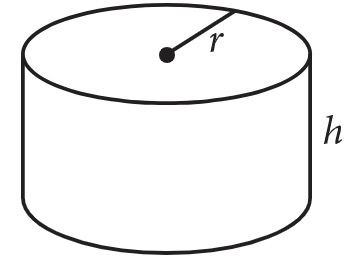
\includegraphics[width=0.54\linewidth]{6.jpg}
\end{center}

The figure shown is a right circular cylinder with a radius of $r$ and height of $h$.  
A second right circular cylinder (not shown) has a volume that is 392 times as large as the volume of the cylinder shown.  
Which of the following could represent the radius $R$, in terms of $r$, and the height $H$, in terms of $h$, of the second cylinder?
\begin{itemize}
    \item[\textbf{A.}] $R = 8r$ and $H = 7h$
    \item[\textbf{B.}] $R = 8r$ and $H = 49h$
    \item[\textbf{C.}] $R = 7r$ and $H = 8h$
    \item[\textbf{D.}] $R = 49r$ and $H = 8h$
\end{itemize}
\end{frame}
\begin{frame}{Answer: The figure shown is a right circular cylinder with a radius of r and hei…}
\textit{Strategy:} Volume scales as $R^2 H$; match the factor $392 = 7\cdot 8^2$ (or equivalent).

\textbf{Correct Answer:} \( \boxed{C} \)

\end{frame}
\begin{frame}{Question: A cube has a volume of 474,552 cubic units}
A cube has a volume of 474{,}552 cubic units.  
What is the surface area, in square units, of the cube?
\end{frame}
\begin{frame}{Answer: A cube has a volume of 474,552 cubic units}
\textit{Strategy:} Percent increase in area: multiply linear scale factors and square.

\textbf{Solution:}
\[ \boxed{36504} \]
\textbf{Correct Answer:} \( \boxed{36504} \)

\end{frame}
\begin{frame}{Question: A right circular cone has a height of 22 centimeters (cm) and a base wit…}
A right circular cone has a height of 22 centimeters (cm) and a base with a diameter of 6 cm.  
The volume of this cone is $n\pi$ cm$^3$. What is the value of $n$?
\end{frame}
\begin{frame}{Answer: A right circular cone has a height of 22 centimeters (cm) and a base wit…}
\textit{Strategy:} Surface area of a cylinder: $2\pi r^2 + 2\pi rh$.

\textbf{Solution:}
\[ \boxed{66} \]
\textbf{Correct Answer:} \( \boxed{66} \)

\end{frame}
\begin{frame}{Question: A manufacturer determined that right cylindrical containers with a heigh…}
A manufacturer determined that right cylindrical containers with a height that is 4 inches longer than the radius  
offer the optimal number of containers to be displayed on a shelf.  
Which of the following expresses the volume, $V$, in cubic inches, of such containers, where $r$ is the radius, in inches?
\begin{itemize}
    \item[\textbf{A.}] $V = 4\pi r^3$
    \item[\textbf{B.}] $V = \pi (2r)^3$
    \item[\textbf{C.}] $V = \pi r^2 + 4\pi r$
    \item[\textbf{D.}] $V = \pi r^3 + 4\pi r^2$
\end{itemize}
\end{frame}
\begin{frame}{Answer: A manufacturer determined that right cylindrical containers with a heigh…}
\textit{Strategy:} Cone volume is $\dfrac{1}{3}$ of a cylinder with the same base and height.

\textbf{Correct Answer:} \( \boxed{D} \)

\end{frame}
\begin{frame}{Question: A rectangular poster has an area of 360 square inches}
A rectangular poster has an area of 360 square inches.  
A copy of the poster is made in which the length and width of the original poster are each increased by 20\%.  
What is the area of the copy, in square inches?
\end{frame}
\begin{frame}{Answer: A rectangular poster has an area of 360 square inches}
\textit{Strategy:} Use $A=\dfrac{1}{2}bh$ or the shoelace formula on the grid.

\textbf{Solution:}
\[ \boxed{25295} \]
\textit{Also accept: 518.4}
\textbf{Correct Answer:} \( \boxed{25295} \)

\end{frame}
\begin{frame}{Question: 28 centimeters (cm)}
A right rectangular prism has a length of \textbf{28 centimeters (cm)},  
a width of \textbf{15 cm}, and a height of \textbf{16 cm}.  
What is the surface area, in cm$^2$, of the right rectangular prism?
\end{frame}
\begin{frame}{Answer: 28 centimeters (cm)}
\textit{Strategy:} Equilateral triangle height: $\dfrac{s\sqrt{3}}{2}$; area $\dfrac{s^2\sqrt{3}}{4}$.

\textbf{Solution:}
\[ \boxed{2216} \]
\textbf{Correct Answer:} \( \boxed{2216} \)

\end{frame}
\begin{frame}{Question: What is the radius, in feet, of the base of the cone?}
A right circular cone has a volume of $\dfrac{1}{3}\pi$ cubic feet and a height of \textbf{9 feet}.  
What is the radius, in feet, of the base of the cone?
\begin{itemize}
    \item[\textbf{A.}] $\dfrac{1}{3}$
    \item[\textbf{B.}] $\dfrac{1}{\sqrt{3}}$
    \item[\textbf{C.}] $\sqrt{3}$
    \item[\textbf{D.}] 3
\end{itemize}
\end{frame}
\begin{frame}{Answer: What is the radius, in feet, of the base of the cone?}
\textit{Strategy:} Similar triangles give proportional sides; set up a ratio.

\textbf{Correct Answer:} \( \boxed{A} \)

\end{frame}
\begin{frame}{Question: Two identical rectangular prisms each have a height of 90 centimeters (c…}
Two identical rectangular prisms each have a height of $90$ centimeters (cm).  
The base of each prism is a square, and the surface area of each prism is $K\ \text{cm}^2$.  
If the prisms are glued together along a square base, the resulting prism has a surface area of $\frac{92}{47}K\ \text{cm}^2$.  
What is the side length, in cm, of each square base?
\begin{itemize}
    \item[\textbf{A.}] $4$
    \item[\textbf{B.}] $8$
    \item[\textbf{C.}] $9$
    \item[\textbf{D.}] $16$
\end{itemize}
\end{frame}
\begin{frame}{Answer: Two identical rectangular prisms each have a height of 90 centimeters (c…}
\textit{Strategy:} Sphere volume formula: $V=\dfrac{4}{3}\pi r^3$.

\textbf{Correct Answer:} \( \boxed{B} \)

\end{frame}
\begin{frame}{Question: The volume of right circular cylinder A is 22 cubic centimeters}
The volume of right circular cylinder $A$ is $22$ cubic centimeters.  
What is the volume, in cubic centimeters, of a right circular cylinder with twice the radius and half the height of cylinder $A$?
\begin{itemize}
    \item[\textbf{A.}] $11$
    \item[\textbf{B.}] $22$
    \item[\textbf{C.}] $44$
    \item[\textbf{D.}] $66$
\end{itemize}
\end{frame}
\begin{frame}{Answer: The volume of right circular cylinder A is 22 cubic centimeters}
\textit{Strategy:} Read the diagram: identify radius and height from labels.

\textbf{Correct Answer:} \( \boxed{C} \)

\end{frame}
\begin{frame}{Question: What is the area, in square units, of the triangle formed by connecting …}
\begin{center}
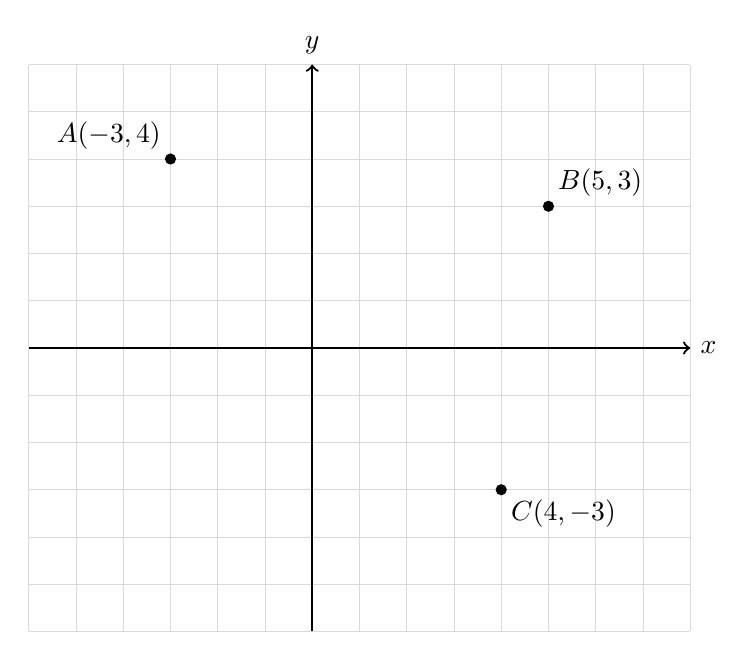
\begin{tikzpicture}[scale=0.6]
    % Draw grid
    \draw[very thin,color=gray!30] (-6,-6) grid (8,6);
    
    % Draw axes
    \draw[->,thick] (-6,0) -- (8,0) node[right] {$x$};
    \draw[->,thick] (0,-6) -- (0,6) node[above] {$y$};

    % Points
    \filldraw[black] (-3,4) circle (3pt) node[above left] {$A(-3,4)$};
    \filldraw[black] (5,3) circle (3pt) node[above right] {$B(5,3)$};
    \filldraw[black] (4,-3) circle (3pt) node[below right] {$C(4,-3)$};


\end{tikzpicture}
\end{center}




What is the area, in square units, of the triangle formed by connecting the three points shown?
\end{frame}
\begin{frame}{Answer: What is the area, in square units, of the triangle formed by connecting …}
\textit{Strategy:} Scale each dimension and apply the volume formula.

\textbf{Solution:}
\[ \boxed{24.5} \]
\textit{Also accept: 49/2}
\textbf{Correct Answer:} \( \boxed{24.5} \)

\end{frame}
\begin{frame}{Question: Circle A has a radius of 3n and circle B has a radius of 129n, where n i…}
Circle $A$ has a radius of $3n$ and circle $B$ has a radius of $129n$, where $n$ is a positive constant.  
The area of circle $B$ is how many times the area of circle $A$?
\begin{itemize}
    \item[\textbf{A.}] $43$
    \item[\textbf{B.}] $86$
    \item[\textbf{C.}] $129$
    \item[\textbf{D.}] $1,849$
\end{itemize}
\end{frame}
\begin{frame}{Answer: Circle A has a radius of 3n and circle B has a radius of 129n, where n i…}
\textit{Strategy:} Right triangle on coordinates: use distance or area formula.

\textbf{Correct Answer:} \( \boxed{D} \)

\end{frame}
\begin{frame}{Question: The dimensions of a right rectangular prism are 4 inches by 5 inches by …}
The dimensions of a right rectangular prism are $4$ inches by $5$ inches by $6$ inches.  
What is the surface area, in square inches, of the prism?
\begin{itemize}
    \item[\textbf{A.}] $30$
    \item[\textbf{B.}] $74$
    \item[\textbf{C.}] $120$
    \item[\textbf{D.}] $148$
\end{itemize}
\end{frame}
\begin{frame}{Answer: The dimensions of a right rectangular prism are 4 inches by 5 inches by …}
\textit{Strategy:} Compare cross-section areas when solids share the same height.

\textbf{Correct Answer:} \( \boxed{D} \)

\end{frame}
\begin{frame}{Question: A right triangle has sides of length 2 2, 6 2, and 80 units}
A right triangle has sides of length $2\sqrt{2}$, $6\sqrt{2}$, and $\sqrt{80}$ units.  
What is the area of the triangle, in square units?
\begin{itemize}
    \item[\textbf{A.}] $8\sqrt{2} + \sqrt{80}$
    \item[\textbf{B.}] $12$
    \item[\textbf{C.}] $24\sqrt{80}$
    \item[\textbf{D.}] $24$
\end{itemize}
\end{frame}
\begin{frame}{Answer: A right triangle has sides of length 2 2, 6 2, and 80 units}
\textit{Strategy:} Composite solid: add/subtract known volumes.

\textbf{Correct Answer:} \( \boxed{B} \)

\end{frame}
\begin{frame}{Question: Triangles ABC and DEF are similar}
Triangles $ABC$ and $DEF$ are similar.  
Each side length of triangle $ABC$ is $4$ times the corresponding side length of triangle $DEF$.  
The area of triangle $ABC$ is $270$ square inches.  
What is the area, in square inches, of triangle $DEF$?
\end{frame}
\begin{frame}{Answer: Triangles ABC and DEF are similar}
\textit{Strategy:} Similarity ratio squared gives the area ratio.

\textbf{Solution:}
\[ \boxed{135/8} \]
\textit{Also accept: 16.87, 16.88}
\textbf{Correct Answer:} \( \boxed{135/8} \)

\end{frame}
\begin{frame}{Question: A cube has a surface area of 54 square meters}
A cube has a surface area of $54$ square meters.  
What is the volume, in cubic meters, of the cube?
\begin{itemize}
    \item[\textbf{A.}] $18$
    \item[\textbf{B.}] $27$
    \item[\textbf{C.}] $36$
    \item[\textbf{D.}] $81$
\end{itemize}
\end{frame}
\begin{frame}{Answer: A cube has a surface area of 54 square meters}
\textit{Strategy:} Plug given dimensions into the correct volume formula.

\textbf{Correct Answer:} \( \boxed{B} \)

\end{frame}

\begin{frame}{}
    \begin{tikzpicture}[remember picture, overlay]
        \shade[top color=novelPurple!40, bottom color=white]
            (current page.north west) rectangle (current page.south east);
        \fill[white, opacity=0.15] (current page.center) circle (5cm);
        \foreach \x in {1,2,3,4,5} {
            \fill[novelPurple, opacity=0.12] (rand*10-5, rand*7-3.5) circle (0.1+\x*0.05);
        }
    \end{tikzpicture}
    \centering
    \vspace{5em}
    {\Huge \textbf{\textcolor{novelPurple}{Thank You!}}} \\[1em]
    {\large \textcolor{gray}{We appreciate your time and focus.}} \\[3em]
    {\LARGE \textbf{\textcolor{novelPurple}{\textsf{Novel Prep}}}}
    \vfill
\end{frame}

\end{document}
